\subsection{Феномен Гіббса та його вплив на інтерполяцію}

Класична теорія наближень базується на фундаментальному принципі: чим більш гладкою є функція, тим швидше збігаються її апроксимації при $n \to \infty$. Проте, коли цільова функція має точки розриву, виникає специфічна математична проблема, відома як феномен Гіббса. У контексті цифрових зображень такі розриви є надзвичайно поширеними — вони відповідають різким перепадам яскравості, контрастним контурам об'єктів та межам текстур.

Історично це явище було вперше описане Генрі Вілбрагамом у 1848 році, проте воно отримало широку відомість після публікацій Джозаї Вілларда Гіббса у 1898–1899 роках. Феномен Гіббса полягає у тому, що при наближенні розривної функції за допомогою рядів Фур'є або поліноміальних інтерполянтів, в околі точок розриву виникають характерні осциляції.

Згідно з сучасними дослідженнями в галузі теорії наближень, зокрема працями Л. Трефетена, феномен Гіббса для поліноміальних інтерполянтів можна розглядати як прямий наслідок поведінки базисних поліномів Лагранжа. Їхні осцилюючі обернено-лінійні «хвости» суттєво впливають на загальний результат інтерполяції в місцях порушення неперервності функції. 

Найбільш критичною особливістю цього явища є те, що зі збільшенням кількості вузлів інтерполяції (тобто зі зростанням ступеня полінома $n$) амплітуда цих викидів не зменшується. Замість цього осциляції стають більш «стиснутими» і просто наближаються впритул до точки розриву. Це свідчить про те, що інтерполяційний процес не забезпечує рівномірної збіжності, незважаючи на поточкову збіжність на гладких ділянках. Наочно ця математична аномалія на прикладі наближення класичної східчастої функції продемонстрована на рис.~\ref{fig:gibbs_phenomenon}.

\begin{figure}[htbp]
	\centering
	% Вкажи правильний шлях до свого файлу gibs.jpg
	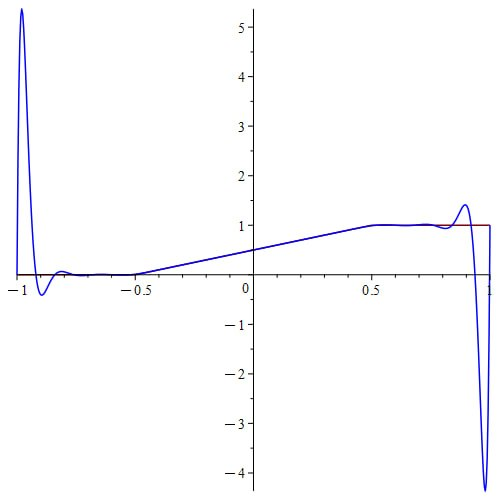
\includegraphics[width=0.6\textwidth]{figures/gibs}
	\caption{Візуалізація феномена Гіббса: збереження амплітуди осциляцій в околі точки розриву незалежно від порядку інтерполяції}
	\label{fig:gibbs_phenomenon}
\end{figure}

\newpage
У задачах просторового масштабування растрових зображень феномен Гіббса має безпосереднє і вкрай негативне практичне значення. Оскільки зображення є дискретними і містять різкі межі, застосування класичної поліноміальної або спектральної інтерполяції високих порядків безпосередньо призводить до появи візуальних дефектів — так званих артефактів «дзвону» (ringing artifacts) або ефекту ореолу навколо контрастних країв. 

Розуміння математичної природи феномена Гіббса є обов'язковою умовою для розв'язання задачі просторового масштабування. Саме це пояснює необхідність розробки спеціальних методів та алгоритмів інтерполяції, які дозволяють мінімізувати ці небажані осциляції та зберегти структурну цілісність зображення при збільшенні його роздільної здатності.